% Chapter 1

\chapter{Introducción general} % Main chapter title

\label{Chapter1} % For referencing the chapter elsewhere, use \ref{Chapter1} 
\label{IntroGeneral}

%----------------------------------------------------------------------------------------

% Define some commands to keep the formatting separated from the content 
\newcommand{\keyword}[1]{\textbf{#1}}
\newcommand{\tabhead}[1]{\textbf{#1}}
\newcommand{\code}[1]{\texttt{#1}}
\newcommand{\file}[1]{\texttt{\bfseries#1}}
\newcommand{\option}[1]{\texttt{\itshape#1}}
\newcommand{\grados}{$^{\circ}$}

%----------------------------------------------------------------------------------------

En este capítulo se introduce la problemática que motivó el presente trabajo, seguida de una breve descripción de la solución propuesta. 
A continuación, se expone el estado del arte de las tecnologías aplicadas. 
Finalmente, se detallan el alcance y los requerimientos necesarios para su implementación.

%----------------------------------------------------------------------------------------
\section{Marco de la propuesta}

En un entorno empresarial, la eficiencia en la búsqueda de información es crucial para la
productividad y el rendimiento de los empleados. Sin embargo, con la creciente cantidad de
datos y documentos disponibles, encontrar información específica de manera rápida y precisa
puede convertirse en un desafío.

La abundancia de fuentes de información, lejos de agilizar el trabajo, a menudo lo complica. En una empresa, 
es común que existan múltiples repositorios de documentos, políticas y datos históricos, pero la falta de centralización y la 
dificultad para identificar la fuente correcta suelen traducirse en pérdidas de tiempo significativas. 
En muchas ocasiones, se dedica más tiempo a la búsqueda de información que a la ejecución de las tareas 
en sí, lo que afecta tanto la productividad como la efectividad en la toma de decisiones.

El presente trabajo surgió como un desarrollo personal para abordar esta problemática. Su propósito fue 
proponer una solución que facilite el acceso ágil y preciso a la información necesaria, de manera tal
que optimice el uso del tiempo en un entorno con gran cantidad de fuentes de información.

Un chatbot especializado ofrece una solución prometedora al permitir a los usuarios realizar 
consultas en lenguaje natural y obtener respuestas de manera instantánea. Mientras que otros sistemas 
de inteligencia artificial ampliamente conocidos y utilizados 
destacan en su capacidad para generar respuestas generales basadas en un amplio conocimiento del 
lenguaje, el presente trabajo se distingue por su capacidad para trabajar con documentos altamente 
específicos (y potencialmente privados). Esto le permite ofrecer respuestas adaptadas al contexto 
interno de la organización, que no podrían obtenerse mediante el uso de los chatbots de 
propósito general disponibles en el mercado \citep{website:chatgpt} \citep{website:copilot} \citep{website:gemini}.

En la figura \ref{fig:diagrama-bloques-basico} se presenta un diagrama de alto nivel de la solución.
En primer lugar, los usuarios interactúan con el chatbot a través de una interfaz gráfica desde donde
pueden realizar consultas sobre la información deseada. Estas consultas, procesadas mediante 
técnicas de lenguaje natural, permiten extraer la información más relevante de la fuente de documentos. 
Luego, un modelo de inteligencia artificial interpreta las consultas y genera respuestas que proporcionan 
al usuario la información solicitada de manera precisa y contextualizada.

\begin{figure}[ht]
	\centering
	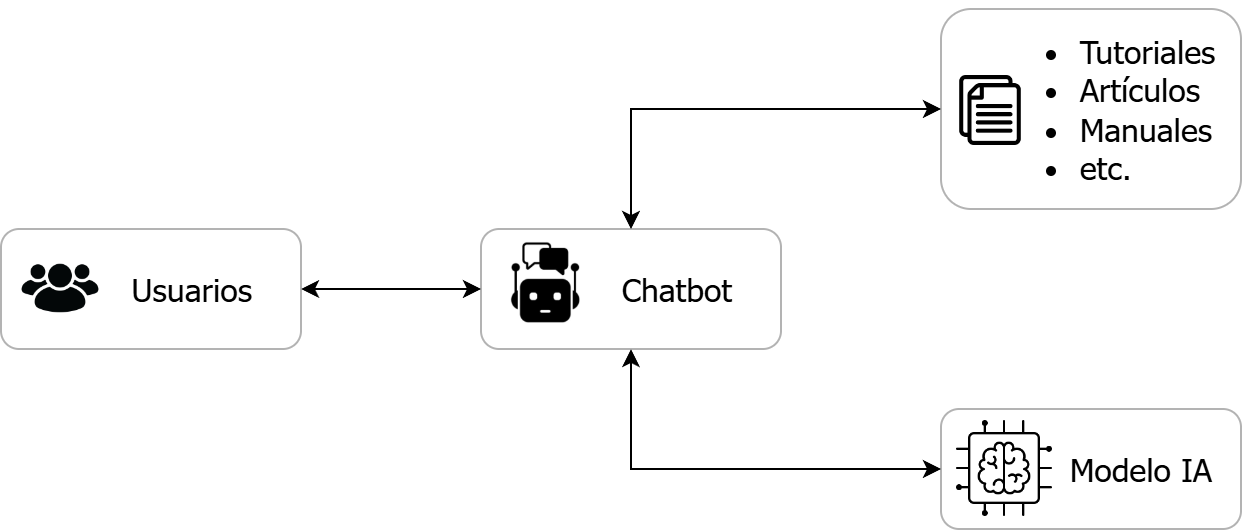
\includegraphics[scale=.3]{./Figures/diagrama_bloques_basico.png}
	\caption{Diagrama de alto nivel de la solución.}
	\label{fig:diagrama-bloques-basico}
\end{figure}

\vspace{15mm}

%----------------------------------------------------------------------------------------
\section{Estado del arte}

El desarrollo de chatbots y sistemas de recuperación de información ha avanzado considerablemente en los últimos años, 
impulsado por mejoras en el procesamiento de lenguaje natural (NLP, por su sigla en inglés) y el acceso a grandes volúmenes de datos. 
En este contexto, los chatbots especializados han surgido como soluciones destacadas para el acceso eficiente 
a información específica en distintos entornos, incluyendo el empresarial. A continuación, se presenta una revisión 
de las principales tecnologías y enfoques actuales que sustentan el desarrollo del presente trabajo.

Los chatbots modernos han evolucionado desde sistemas de reglas simples hasta modelos sofisticados capaces de 
mantener conversaciones complejas. Entre los primeros desarrollos, como ELIZA \citep{paper:eliza} en 
la década de 1960, se empleaban reglas predefinidas que limitaban la interacción a una cantidad pequeña de 
respuestas posibles. Sin embargo, el uso de redes neuronales y el aprendizaje profundo en las últimas décadas 
han revolucionado el campo, al permitir la aparición de sistemas como Siri de Apple, Alexa de Amazon 
y Google Assistant \citep{article:voice-assistants}. Estos asistentes virtuales han popularizado el uso de interfaces 
de conversación en la vida cotidiana, ya que son capaces de responder a preguntas comunes, realizar tareas administrativas 
y ofrecer asistencia en tiempo real.

Una tendencia reciente en el desarrollo de chatbots es la aplicación de modelos generativos de lenguaje, como GPT-3 y GPT-4 
de OpenAI \citep{paper:gpt}, BERT de Google \citep{paper:bert}, y LLAMA de Meta \citep{paper:llama}. Estos modelos, basados 
en arquitecturas de \textit{transformers} \citep{paper:transformers}, permiten una comprensión profunda del contexto y del 
significado en secuencias de palabras. Su capacidad de generar respuestas coherentes y bien estructuradas ha llevado al 
desarrollo de los tan populares chatbots modernos como ChatGPT \citep{website:chatgpt}, Microsoft Copilot \citep{website:copilot}
o Google Gemini \citep{website:gemini}, cuyas interfaces se observan en la figura \ref{fig:chatbots}.

\vspace{25mm}

\begin{figure}[ht]
	\centering
	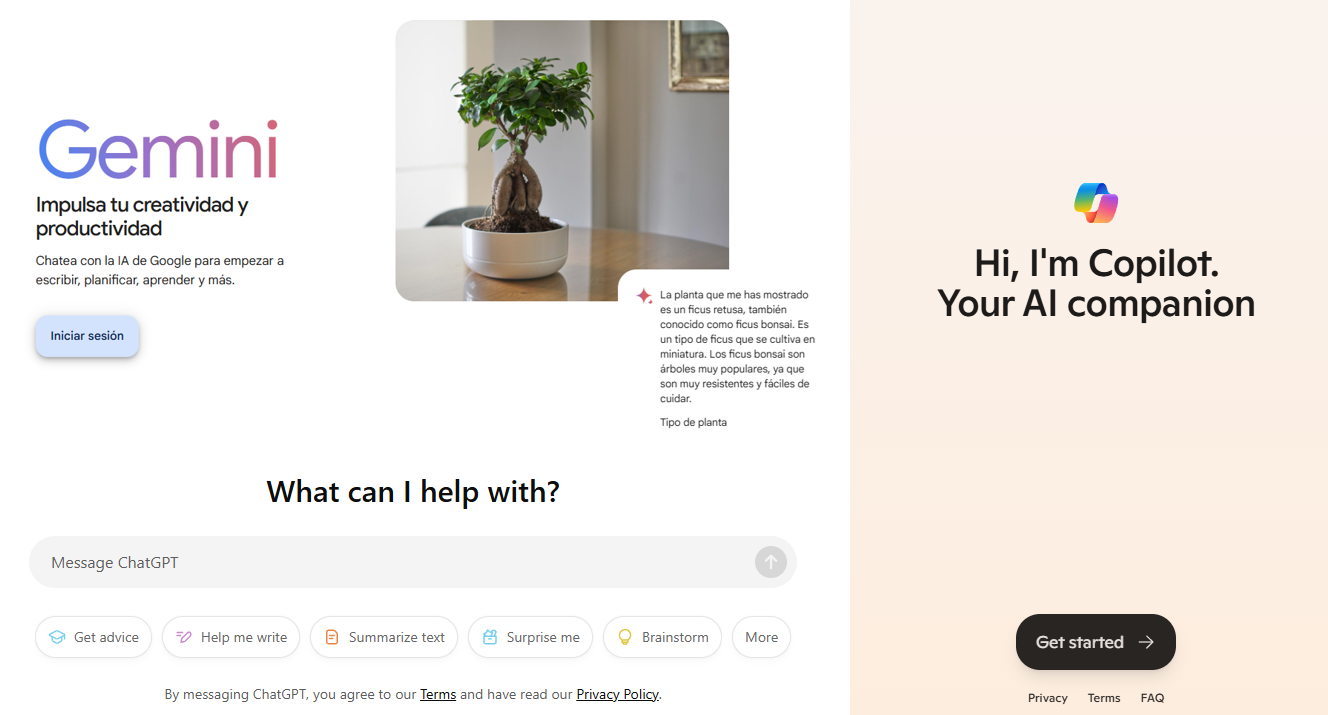
\includegraphics[scale=.38]{./Figures/chatbots.png}
	\caption{ChatGPT, Gemini y Copilot, los chatbots más populares actualmente.}
	\label{fig:chatbots}
\end{figure}

\vspace{10mm}

Si bien los modelos generativos han alcanzado un alto grado de sofisticación, presentan algunas limitaciones importantes. 
En primer lugar, su conocimiento es en gran medida de propósito general, dado que han sido entrenados con grandes volúmenes 
de datos públicos y no específicos, lo que limita su precisión cuando se requiere información particular de una organización. 
En segundo lugar, estos modelos tienden a ``inventar'' respuestas cuando no encuentran información relevante, fenómeno conocido 
como \textit{hallucinations} \citep{article:hallucinations}. En un contexto empresarial, esto puede provocar confusión o incluso 
proporcionar información errónea.

En la búsqueda de soluciones que combinen la capacidad de los modelos generativos con la precisión de la información propietaria, 
ha surgido el enfoque de generación aumentada por recuperación (RAG, por su sigla en inglés). Este enfoque combina sistemas de 
recuperación de información con modelos de generación de texto, lo que permite que las respuestas no solo se basen en la capacidad 
generativa del modelo, sino también en una búsqueda previa en bases de datos o documentos específicos \citep{paper:rag-1} 
\citep{paper:rag-2}.

El presente trabajo se apoya en el estado del arte de los modelos de lenguaje y la técnica de RAG para crear una solución innovadora.

\vspace{10mm}

%----------------------------------------------------------------------------------------
\section{Objetivos y alcance}

El propósito de este trabajo fue optimizar el proceso de búsqueda de información por parte de los empleados. Se buscó
proporcionar una herramienta eficaz que permita acceder rápidamente a los datos relevantes, que mejore la eficiencia y 
productividad en el entorno laboral.

Para ello, se realizaron las siguientes tareas:

\begin{itemize}
	\item Procesamiento de los documentos y posterior almacenamiento en una base de datos.
	\item Integración con un modelo lingüístico grande (LLM) que pueda entender las consultas de los usuarios y proporcionar respuestas precisas basadas en el contenido de los documentos ingestados.
	\item Diseño e implementación de una interfaz de usuario intuitiva y fácil de utilizar que permita a los empleados interactuar con el chatbot de manera eficiente.
	\item Desarrollo de un \textit{pipeline} de despliegue continuo que facilite la ingesta de nuevos documentos y la actualización de la aplicación.
  \item Evaluación del rendimiento del chatbot mediante pruebas exhaustivas con diferentes tipos de consultas.
\end{itemize}

\vspace{5mm}

Las siguientes actividades no formaron parte del alcance:

\begin{itemize}
	\item Despliegue del chatbot en un ambiente productivo.
	\item Entrenamiento continuo del chatbot en base a las consultas realizadas por los usuarios.
	\item Desarrollo de funcionalidades avanzadas de seguridad, tales como autenticación de usuarios o cifrado de datos.
\end{itemize}

\vspace{10mm}

%----------------------------------------------------------------------------------------
\section{Requerimientos}

A continuación se describen los principales requerimientos establecidos durante la etapa de planificación:

\begin{enumerate}
	\item Requerimientos funcionales:
		\begin{enumerate}
			\item El sistema debe permitir a los usuarios consultar por información a través de una interfaz gráfica.
			\item El sistema debe ser capaz de entender consultas escritas en lenguaje natural.
			\item El sistema debe proporcionar respuestas precisas basadas en el contenido de los documentos procesados.
		\end{enumerate}
	\item Requerimientos de la interfaz:
		\begin{enumerate}
	  		\item La interfaz gráfica debe ser intuitiva y fácil de usar para los usuarios.
	  		\item Se debe proporcionar retroalimentación instantánea al usuario luego de realizar una consulta.
	  	\end{enumerate}
	\item Requerimiento de testing:
	  	\begin{enumerate}
	  		\item Se deben realizar pruebas exhaustivas para garantizar la precisión y la robustez del sistema.
	  	\end{enumerate}
	\vspace{10mm}
	\item Requerimientos de documentación:
		\begin{enumerate}
			\item Se deben documentar las pruebas realizadas y los resultados obtenidos.
			\item Se debe elaborar un informe de avance del proyecto.
			\item Se debe confeccionar una memoria técnica del proyecto.
		\end{enumerate}
	\item Requerimientos de cumplimiento normativo:
		\begin{enumerate}
			\item El sistema debe cumplir con las regulaciones de privacidad de datos vigentes.
		\end{enumerate}
\end{enumerate}